\documentclass[12pt]{article}

\usepackage{sbc-template}
\usepackage{graphicx,url}
\usepackage[english]{babel}
\usepackage[utf8]{inputenc}
\usepackage{amsmath}
\usepackage[pdftex]{hyperref}

%\usepackage[brazil]{babel}   
\usepackage[utf8]{inputenc}  

% Pacote para a definição de novas cores
\usepackage{xcolor}
% Definindo novas cores
\definecolor{verde}{rgb}{0.25,0.5,0.35}
\definecolor{jpurple}{rgb}{0.5,0,0.35}
\definecolor{darkgreen}{rgb}{0.0, 0.2, 0.13}
%\definecolor{oldmauve}{rgb}{0.4, 0.19, 0.28}
% Configurando layout para mostrar codigos Java
\usepackage{listings}

\newcommand{\estiloJava}{
\lstset{
    language=Java,
    basicstyle=\ttfamily\small,
    keywordstyle=\color{jpurple}\bfseries,
    stringstyle=\color{red},
    commentstyle=\color{verde},
    morecomment=[s][\color{blue}]{/**}{*/},
    extendedchars=true,
    showspaces=false,
    showstringspaces=false,
    numbers=left,
    numberstyle=\tiny,
    breaklines=true,
    backgroundcolor=\color{cyan!10},
    breakautoindent=true,
    captionpos=b,
    xleftmargin=0pt,
    tabsize=2
}}
     
\sloppy

\title{Sintaxe e Semântica em Dart\\ Linguagens de Programação}

\author{Lucas Carvalho da Luz\inst{}, João Pedro Barroso Da Silva Neto\inst{}, Lucas Vinícius S. G. Coelho\inst{}}

\address{ICEI -- Pontifícia Universidade Católica de Minas Gerais
  (PUC)\\
  Rua Claudio Manuel, 1.162 – Funcionarios – Belo Horizonte – MG – Brazil
\email{\{lcluz\}@sga.pucminas.br, \{lucas.coelho.1324003\}@sga.pucminas.br},
\email{\{joao.neto.1313048\}@sga.pucminas.br}
}

\begin{document} 
\maketitle
\begin{resumo} 
  Esse texto e um guia introdutório da linguagem Dart, com o intuito de brevemente explicar
os conteudos de aplicações, estrutura de dados, tipos, paradigmas, estruturas de controle,
funções e topicos avançados, como concorrência e paralelismo, presentes na linguagem.
O repositorio da aplicação pratica esta localizado no Github, no qual o arquivo
contendo o codigo: main.dart, e o vıdeo final no YouTube.

\end{resumo}

\section{Domínios de Aplicação}
Dart é uma linguágem primariamente, desenvolvimento de aplicações com foco client-side devido à sua adoção pelo framework de desenvolvimento front-end Flutter. Porém, serve também para o desenvolvimento de aplicações server-side.

\section{Tipos de Dados e Sistemas de Tipos}
Um benefício dessa checagem estática é a capacidade de encontrar problemas em tempo de compilação, e é possível consertar a maior parte dos erros capturados por ela adicionando anotações de tipo à classes genéricas, como listas ( List $<T>$ ) e mapas ( Map $<K,V>$ ).

\subsection{built in types}
Dart já vem vários tipos integrados, como:
\begin{itemize}
    \item int, double
    \item String
    \item bool
    \item List
    \item Set
    \item Map
    \item Runes
    \item Symbol
    \item null
    \item Future, Stream
    \item Never
    \item dynamic
    \item void
\end{itemize}

Todos eles exceto o Null, são subclasses da classe object

\section{Alocação de Memória}
Em Dart é possível alocar memória estaticamente com a palavra chave static (só são inicializadas quando são utilizadas), tanto de variáveis como de métodos.

Os métodos estáticos não operam em uma instância, no entanto, eles têm acesso a variáveis estáticas e podem ser passados como parâmetro.

Métodos de instâncias funcionam de forma similar a de métodos estáticos, tirando a parte de serem estáticos, e pertencem a um objeto. Ambos são métodos normais, possuem tipos, podem ser chamados, e podem ser passados como parâmetro como qualquer outro valor.

Objetos instanciados vivem na heap, que é gerenciada pela Dart VM, que é a máquina virtual do Dart que gerencia a execução e a memória do programa.

O coletor de lixo que é utilizado pela Dart VM para fazer a limpeza da memória trata a heap em busca de regiões de memória não mais utilizadas, permitindo a melhor reutilização da memória do programa e reduzindo problemas relacionados ao uso de memória. Esse processo é feito automaticamente pela VM.

\section{Principais instruções de controle}
Dart possui as seguintes instruções de controle:

\begin{itemize}
    \item if e else
    \item for, while e do while
    \item break e continue
    \item switch e case
    \item assert
    \item try, catch, throw e finally
\end{itemize}

    O funcionamento delas não difere muito do que é visto em C ou C++, com exceção do assert,
que é um mecanismo de checagem de consistência usado na fase de desenvolvimentopara notificar
a utilização incorreta de alguma classe.

\begin{scriptsize}
\estiloJava
\begin{lstlisting}[caption={}, label=lst:javacode1]
// Make sure the variable has a non-null value.
assert(text != null);

// Make sure the value is less than 100.
assert(number < 100);

// Make sure this is an https URL.
assert(urlString.startsWith('https'));

\end{lstlisting}
\end{scriptsize}

\section{Sinxtaxe e expressividade}
Dart apresenta uma sintaxe semelhante à de Java, JavaScript e C# devido a similaridades como a forma de fazer anotações e nomenclatura e estrutura de classes e tipos, nomes de métodos existentes em tipos e classes embutidos na linguagem e conceitos que a linguagem aplica.

Um exemplo disso são métodos utilitários presentes em classes em geral, como map, a forma que é possível declarar valores de um certo tipo utilizando literals bem similares à forma como é feito em JavaScript, e também a sintaxe de declaração de lambdas.


\section{Recursividade}
Dart suporta recursividade como qualquer outra linguagem que também suporta.
\begin{scriptsize}
\estiloJava
\begin{lstlisting}[caption={}, label=lst:javacode10]
 void main() {
  func(10);
}

void func(int n) {
  if (n <= 0) return;
  
  return func(--n);
}


\end{lstlisting}
\end{scriptsize}

\begin{scriptsize}
\estiloJava
\begin{lstlisting}[caption={}, label=lst:javacode11]
 class Coisa {
  final Coisa? coisa;
  
  const Coisa(this.coisa);
}

\end{lstlisting}
\end{scriptsize}

\section{Concorrência}
As palavras chave async e await têm significado especial na linguagem Dart, e permitem uma
maneira declarativa de definir funções assíncronas.

Em termos práticos, é possível dar await em uma função que retorne uma Future, mas somente
dentro de uma função que seja async. Para definir uma função assíncrona, adicione a palavra
chave async antes da declaração do corpo da função.

\begin{scriptsize}
\estiloJava
\begin{lstlisting}[caption={}, label=lst:javacode2]
String createOrderMessage() {
  var order = fetchUserOrder();
  return 'Your order is: $order';
}

Future<String> fetchUserOrder() =>
    // Imagine that this function is
    // more complex and slow.
    Future.delayed(
      const Duration(seconds: 2),
      () => 'Large Latte',
    );

void main() {
  print('Fetching user order...');
  print(createOrderMessage());
}
\end{lstlisting}
\end{scriptsize}

Quanto à concorrência, muitos programas desenvolvidos em Dart utilizam de somente um isolate, que atua como o principal processo que roda a aplicação, mas é possível criar vários isolates, permitindo a execução de código em paralelo utilizando múltiplos cores.

\section{Paradigmas de programação presentes}
Dart é uma linguagem orientada a objetos e apresenta aspectos dos paradigmas funcional, orientado a objetos e imperativo. Apresenta conceitos de orientação a objeto e mixins. Cada objeto é uma instância de uma classe, e todas as classes, exceto Null, descendem de Object.
Quando você chama um método, você o invoca em um objeto: o método tem acesso às funções e dados desse objeto

\section{Null safety}
Em Dart as variáveis são não anuláveis, entretanto é possível adicionar ? para aceitar valores nulos.

\begin{scriptsize}
\estiloJava
\begin{lstlisting}[caption={}, label=lst:javacode3]
var i = 42;
String name = getFileName();
final b = Foo();
ou 
int? nullInt = null;

\end{lstlisting}
\end{scriptsize}

\begin{figure}[!htb]
    \centering
    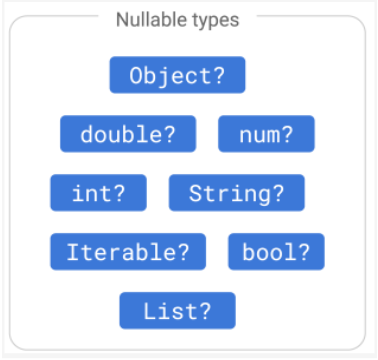
\includegraphics[width=.4\textwidth]{unknown (1).png}
    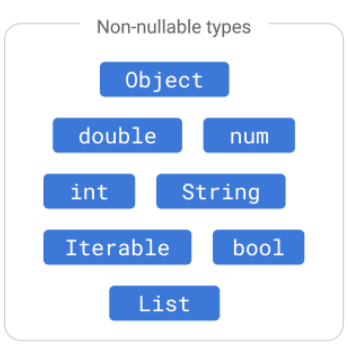
\includegraphics[width=.4\textwidth]{unknown (2).png}
\end{figure}

\section{Parâmetros}

Dart tem 2 tipos de parâmetros: posicionais e nomeados. Parâmetros posicionais são o tipo de parâmetro que são comumente vistos em outras linguagens:

\begin{scriptsize}
\estiloJava
\begin{lstlisting}[caption={}, label=lst:javacode4]
int sumUp(int a, int b, int c) {
  return a + b + c;
}
// ···
  int total = sumUp(1, 2, 3);
\end{lstlisting}
\end{scriptsize}

É possível fazer com que parâmetros sejam opcionais colocando-os entre colchetes, e eles têm
sempre que vir por último na lista de parâmetros:

\begin{scriptsize}
\estiloJava
\begin{lstlisting}[caption={}, label=lst:javacode5]
int sumUpToFive(int a, [int? b, int? c, int? d, int? e]) {
  int sum = a;
  if (b != null) sum += b;
  if (c != null) sum += c;
  if (d != null) sum += d;
  if (e != null) sum += e;
  return sum;
}
// ···
  int total = sumUpToFive(1, 2);
  int otherTotal = sumUpToFive(1, 2, 3, 4, 5);
\end{lstlisting}
\end{scriptsize}

Utilizando chaves, é possível definir parâmetros que funcionam a partir de nomes.

\begin{scriptsize}
\estiloJava
\begin{lstlisting}[caption={}, label=lst:javacode6]
void printName(String firstName, String lastName, {required String suffix}) {
  print('$firstName $lastName $suffix');
}
// ···
  printName('Avinash', 'Gupta');
  printName('Poshmeister', 'Moneybuckets', suffix: 'IV');

\end{lstlisting}
\end{scriptsize}

É possível também fazer estes parâmetros serem obrigatórios utilizando a palavra chave required.

\begin{scriptsize}
\estiloJava
\begin{lstlisting}[caption={}, label=lst:javacode7]
void printName(String firstName, String lastName, {String? suffix}) {
  print('$firstName $lastName ${suffix ?? ‘’}');
}
// ···
  printName('Avinash', 'Gupta');
  printName('Poshmeister', 'Moneybuckets', suffix: 'IV');
\end{lstlisting}
\end{scriptsize}


\section{Modificadores de acesso}
Em Dart, não existem identificadores de acesso como public ou private. Em vez de utilizar essas palavras chave, a linguagem utiliza de uma outra lógica, que envolve a utilização do caractere (\_) antes do nome da variável, o que torna ela private - caso contrário ela é public.

Essa lógica também vale para a exportação de membros entre arquivos: um identificador iniciado com (\_) não poderá ser importado por outros arquivos.

\section{Construtores}
Em Dart é possível usar atalhos para criação de construtores, como o this.propertyName 
para declarar o construtor, e criação de múltiplos construtores
\begin{scriptsize}
\estiloJava
\begin{lstlisting}[caption={}, label=lst:javacode8]
class MyColor {
  int red;
  int green;
  int blue;

  MyColor(this.red, this.green, this.blue);
  MyColor.black()
      : red = 0,
        green = 0,
        blue= 0;
}
final color = MyColor(80, 80, 128);
final blackColor = MyColor.black();
\end{lstlisting}
\end{scriptsize}

Em alguns casos é  possível também utilizar o required para impedir valores nulos ou colocar um valor default
\begin{scriptsize}
\estiloJava
\begin{lstlisting}[caption={}, label=lst:javacode9]
 MyColor({required this.red, required this.green, required this.blue});
ou
  MyColor([this.red = 0, this.green = 0, this.blue = 0]);
\end{lstlisting}
\end{scriptsize}

\section{Plataformas}
Flutter tem suporte a várias plataformas como a Web, Android, iOS, Windows e Linux. O que isso significa é que com ele é possível fazer aplicativos que rodam no navegador, em celulares, e como aplicações desktop também.


\bibliographystyle{sbc}
\bibliography{sbc-template}

\url{https://dart.dev/}; 

\url{https://youtu.be/GA9tNAp1itE/};

\url{https://github.com/LucasVinicius314/lp-linguagem};

\end{document}
